%ju 28-Mai-22 FM_U03_Reihenschaltung_Loesung.tex
\section{Reihenschaltung Übung 3}\label{reihenschaltung-uebung-3}

\textbf{Aufgabe 1}

geg:

$R_1 = 40~\Omega, R_2 = 110~\Omega, R_3 = 50~\Omega$

$U_2 = 4,4~V$

ges: $I, U_1, U_3$

Formel

$I = \frac{U_2}{R_2}$

$U_1 = R_1 \cdot I, U_3 = R_3 \cdot I$

Lösung:

$I = 0,04~A$

$U_1 = 1,6~V, U_3 = 2,0~V$

\textbf{Aufgabe 2}

geg:

$R_1 = 8~\Omega, R_2 = 24~\Omega$

$U_{ges} = 12~V$

$I = 0,27~A = 270~mA$

ges: $R_{ges}, R_3, U_1, U_2, U_3$

Formel

$R_{ges} = \frac{U_{ges}}{I}$

$R_{ges} = R_1 + R_2 + R_3 \to R_3 = R_{ges} - R_1 - R_2$

$U_1 = R_1 \cdot I, U_2 = R_2 \cdot I, U_3 = R_3 \cdot I$

Lösung:

$R_{ges} = 44,4444~\Omega, R_3 = 12,4444~\Omega$

$U_1 = 2,16~V, U_2 = 6,48~V, U_3 = 3,36~V$

\newpage

\textbf{Aufgabe 3}

\begin{figure}[!ht]% hier: !ht
\centering
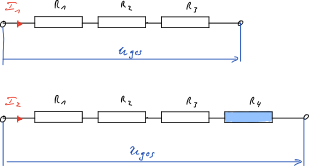
\includegraphics[width=0.6\textwidth]{images/Skizze/22_FM_Nr3_Reihenschaltung_Aufg3_Skizze.pdf}
\caption{Schaltung Reihenschaltung Aufgabe 3}
%\label{fig:}%% anpassen
\end{figure}

geg:

$R_1 = R_2 = R_3 = 22~\Omega$

$I_1 = 0,87~A = 870~mA$

$I_{delta} = 0,075~A = 75~mA$

ges: $I_2, R_{ges_1}, U_{ges}, R_{ges_2}, R_4, U_1, U_2, U_3, U_4$

Formel

$I_2 = I_1 - I_{delta}$

$R_{ges_1} = R_1 + R_2 + R_3$

$U_{ges} = R_{ges_1} \cdot I_1$

$R_{ges_2} = \frac{U_{ges}}{I_2}$

$R_{ges_2} = R_1 + R_2 + R_3 + R_4 \to R_4 = R_{ges_2} - R_1 - R_2 - R_3$

$U_4 = R_4 \cdot I_2$

$U_1 = R_1 \cdot I_2$

Lösung:

$I_2 = 0,795~A$

$R_{ges1} = 66~\Omega$

$U_{ges} = 57,42~V$

$R_{ges2} = 72,2264~\Omega$

$R_4 = 6,2264~\Omega$

$U_4 = 4,95~V$

$U_1 = 17,49~V \to R_1 = R_2 = R_3 \to U_1 = U_2 = U_3$

\newpage

\textbf{Aufgabe 4}

\begin{figure}[!ht]% hier: !ht
\centering
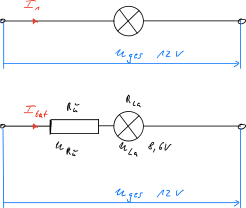
\includegraphics[width=0.6\textwidth]{images/Skizze/23_FM_Nr3_Reihenschaltung_Aufg4_Skizze.pdf}
\caption{Schaltung Reihenschaltung Aufgabe 4}
%\label{fig:}%% anpassen
\end{figure}

geg:

$U_{ges} = 12~V$

$I_1 = 1,75~A$

$U_{La} = 8,6~V$

ges: $U_{R_\text{ü}}, R_{La}, I_{tat}, R_\text{ü}$

Formel

$U_{ges} = U_{La} + U_{R_\text{ü}} \to U_{R_\text{ü}} = U_{ges} - U_{La}$

$R_{La} = \frac{U_{ges}}{I_1}$

$I_{tat} = \frac{U_{La}}{R_{La}}$

$R_\text{ü} = \frac{U_{R_\text{ü}}}{I_{tat}}$

Lösung:

$U_{R_\text{ü}} = 3,4~V$

$R_{La} = 6,8571~\Omega$

$I_{tat} = 1,2542~A$

$R_\text{ü} = 2,711~\Omega$
